\documentclass{beamer}
\usepackage[T1]{fontenc}
\usepackage[utf8]{inputenc}
\usepackage[french]{babel}
\usetheme{Berlin}

\title{Conception et développement multi-lots / multi-équipes\\ \emph{Application à la supervision à distance d'une ligne de conditionnement temps réel}}
\author{Hexanôme 4203\\ Etienne \textsc{Brodu} Martin \textsc{Richard} Maxime \textsc{Gaudin}\\ Monica \textsc{Golumbeanu} Paul \textsc{Adenot} Yoann \textsc{Rodière}}

\begin{document}

	\begin{frame}
		\titlepage
	\end{frame}

\section{Introduction}
	\begin{frame}
		\begin{itemize}	
			\item Voyants
			\item Impression des étiquettes %Charge des imprimantes
			\item Journal d'exploitation
			\item Client Windows
			\item Erreurs et Anomalies
			\item Protocole
			%TODO Est-ce bien nécessaire de tout détailler ?
		\end{itemize}
	\end{frame}

	\begin{frame}
		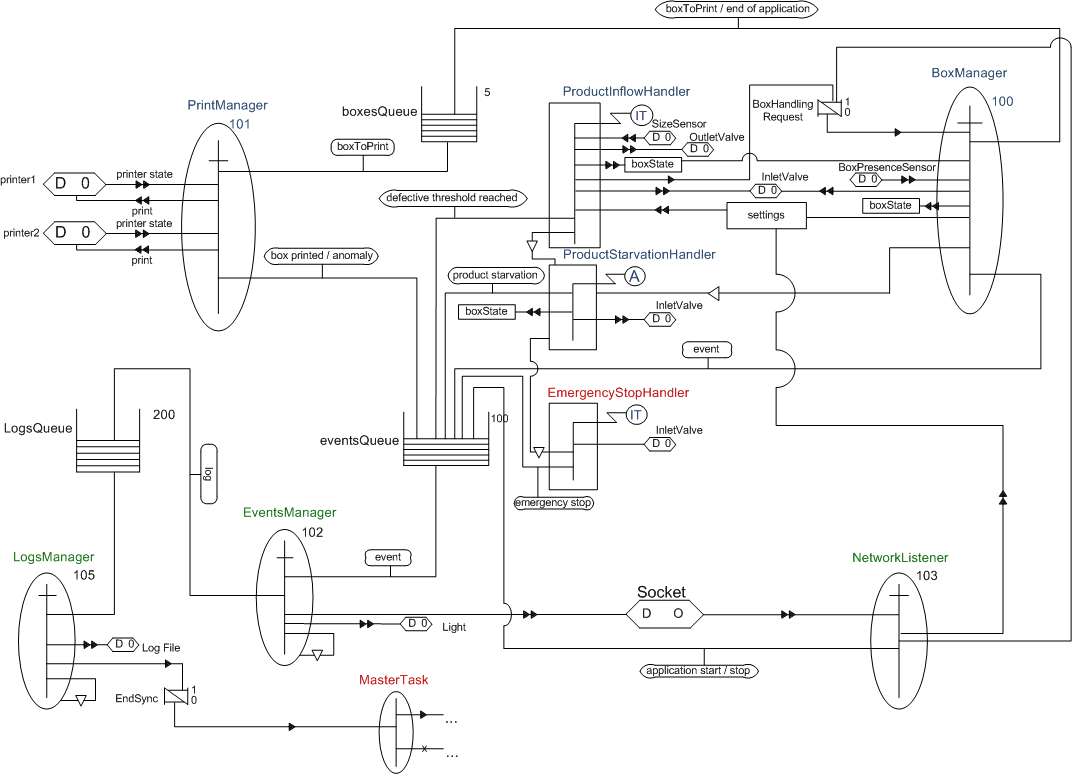
\includegraphics[width=\textwidth]{../../SchemasLCG/schemaGlobal.png}
		%TODO Découpage en lot fonctionnel.
	\end{frame}

	\begin{frame}
		IHM du poste distant
		connection
	\end{frame}

	\begin{frame}
		IHM du poste distant
		configuration
	\end{frame}

	\begin{frame}
		IHM du poste distant
		log
	\end{frame}

	\begin{frame}
		IHM du poste distant
		erreur \/ warning
	\end{frame}

\section{Binôme 1 (Monica, Yoann)}
	\begin{frame}
	\begin{center}
		\huge Lot 1 : partie métier
		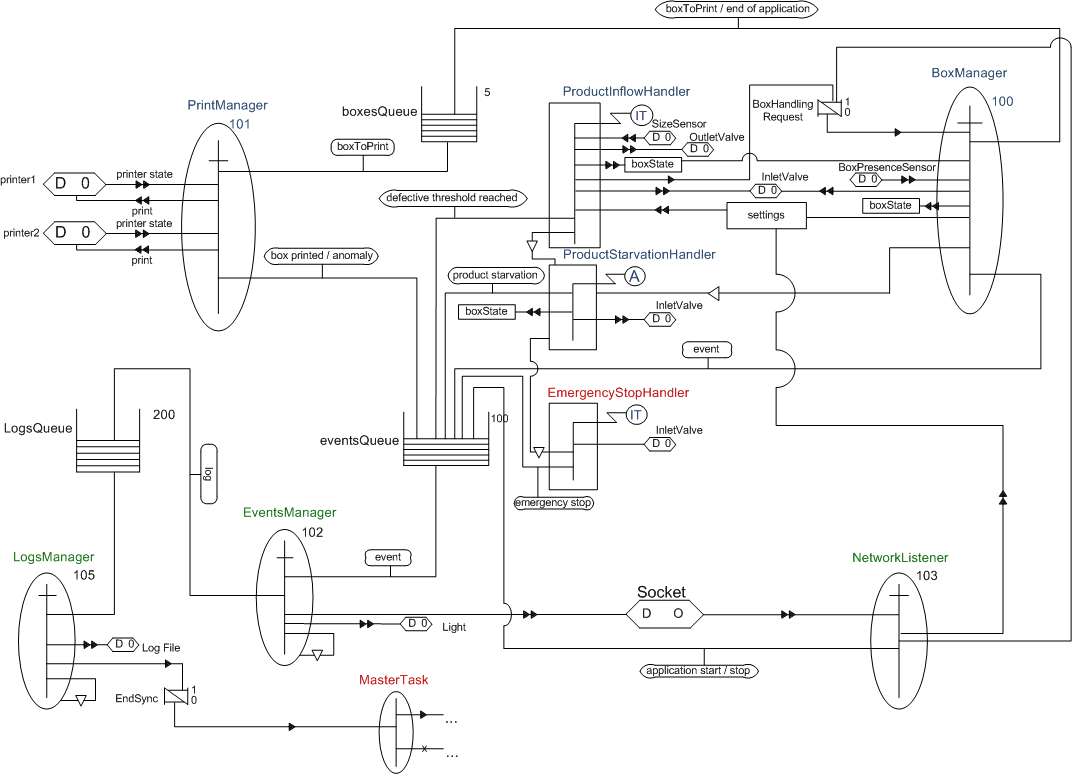
\includegraphics[height=0.8\textheight]{../../SchemasLCG/schemaGlobal.png}
	\end{center}
	\end{frame}

\subsection{Gestion du remplissage}
	\begin{frame}
	\begin{figure}
		\centering
		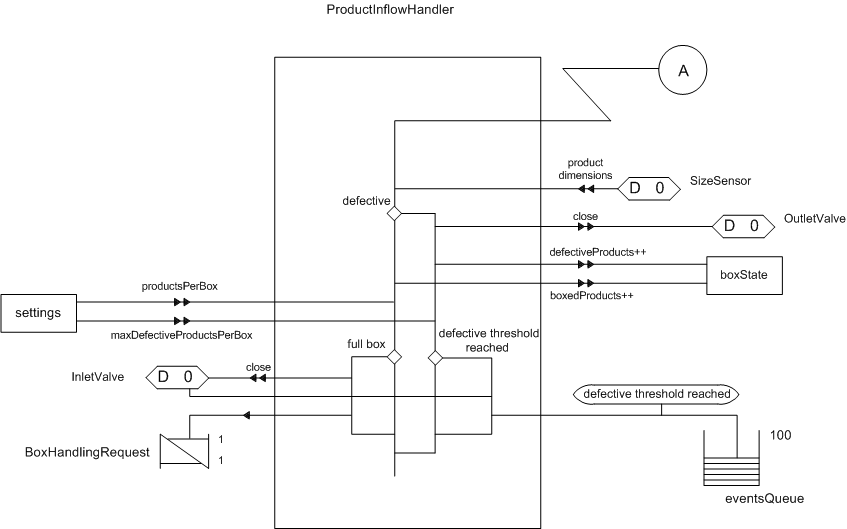
\includegraphics[width=0.9\textwidth]{../../SchemasLCG/ProductInflowHandler.png}
	\end{figure}
	\end{frame}

	\begin{frame}
	\begin{figure}
		\centering
		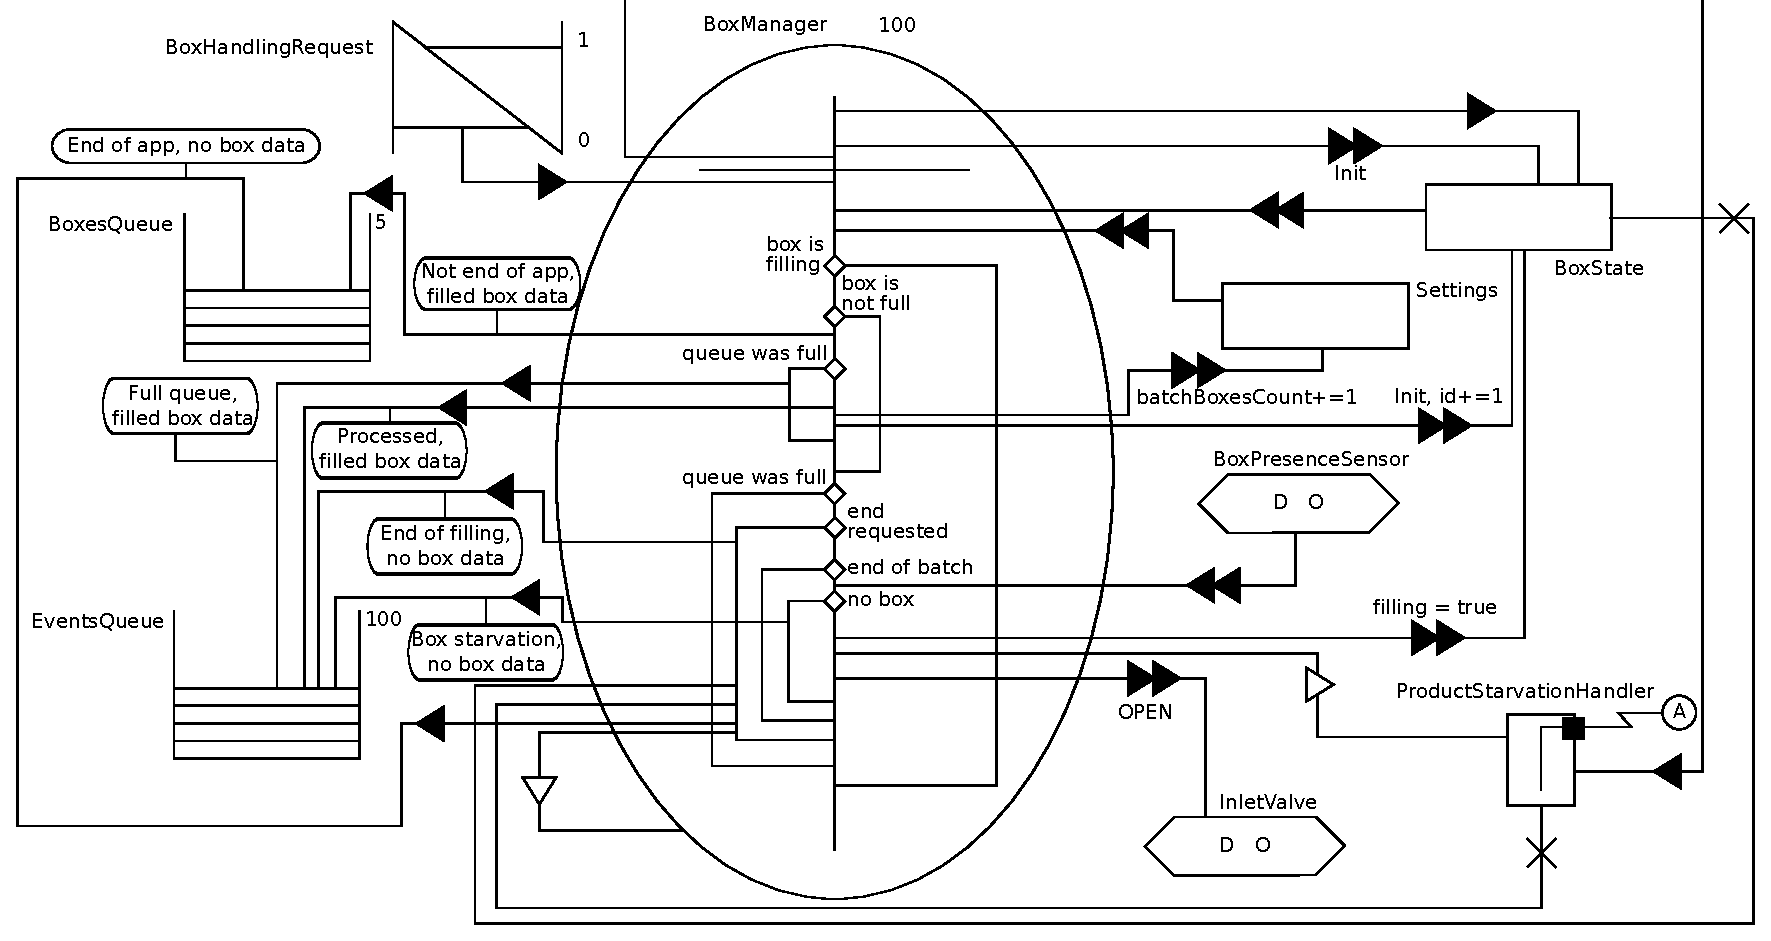
\includegraphics[width=\textwidth]{../../SchemasLCG/BoxManager.pdf}
	\end{figure}
	\end{frame}

	\begin{frame}
	\begin{figure}
		\centering
		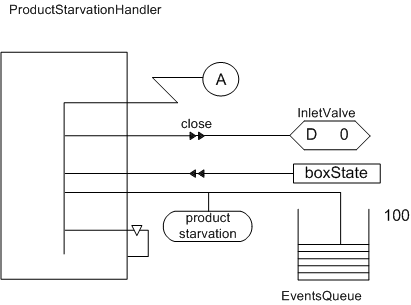
\includegraphics[width=0.7\textwidth]{../../SchemasLCG/ProductStarvationHandler.png}
	\end{figure}
	\end{frame}

\subsection{Gestion de l'impression}
	\begin{frame}
	\begin{figure}
		\centering
		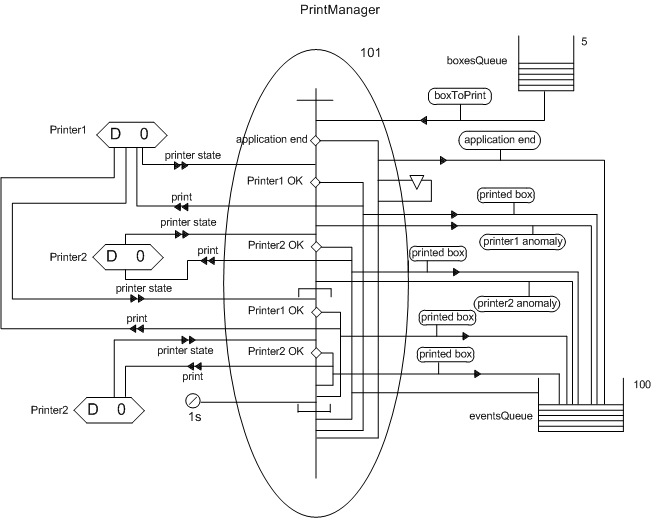
\includegraphics[width=0.85\textwidth]{../../SchemasLCG/PrintManager.png}
	\end{figure}
	\end{frame}

\section{Binôme 2 (Paul, Maxime)}
	\begin{frame}
	\begin{center}
		\huge Lot 2 : TODO décrire
		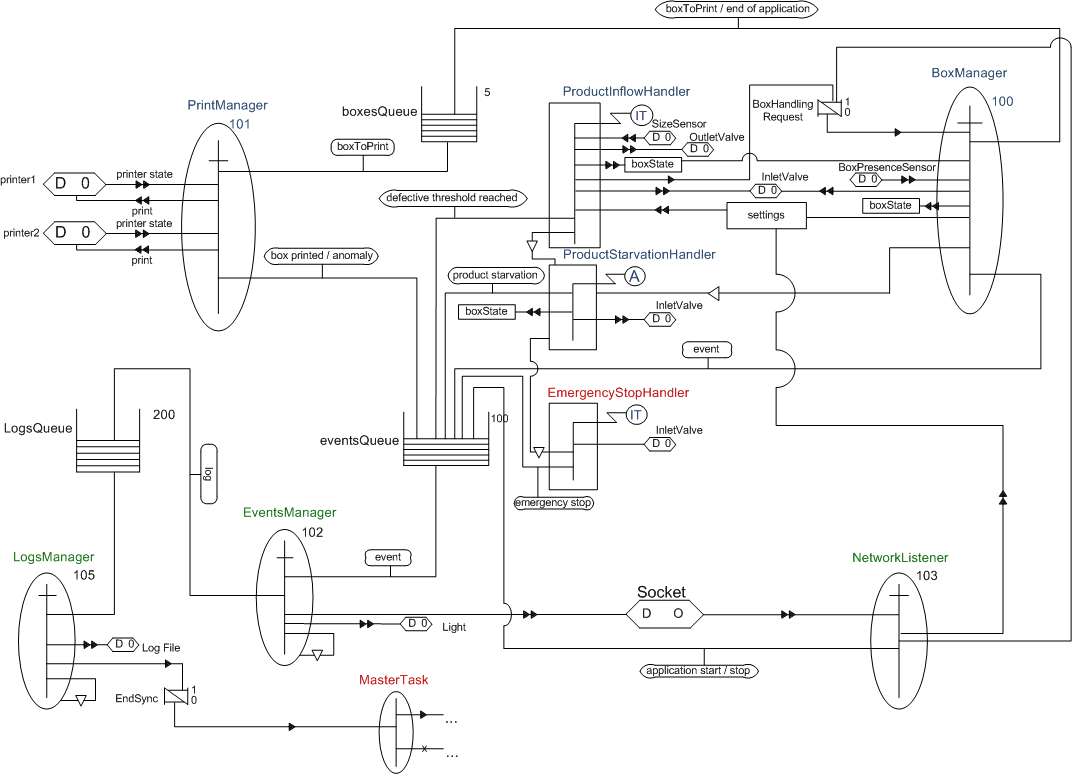
\includegraphics[height=0.8\textheight]{../../SchemasLCG/schemaGlobal.png}
	\end{center}
	\end{frame}

	\begin{frame}

	\frametitle{Lot 2 : réseau, journalisation, gestion des évènements.}

	    \begin{block}{Réalisé par Paul et Maxime}

	  \begin{itemize}

	      \item   Communication réseau en entrée et en sortie du système.

	      \item   Communication des évènements par boite aux lettres à

	      l'intérieur du système.

	      \item   Gestion de la journalisation sur disque.

	  \end{itemize}

	    \end{block}

	\end{frame}

	

	\begin{frame}

	\frametitle{Protocole}

	    \begin{block}{Choix}

	  \begin{itemize}

	      \item Protocole \texttt{plain text}.

	      \item Séparateur : retour chariot.

	      \item 9 commandes différentes dans les deux sens.

	  \end{itemize}

	    \end{block}

	\end{frame}

	

	\begin{frame}

	\frametitle{Protocole en entrée}

	\begin{enumerate}

	    \item \texttt{RESUME} : reprise sur erreur.

	    \item \texttt{STOP} : arrêt du système après les cartons courants.

	    \item \texttt{CONFIG} : 5 valeurs chiffrées pour configurer le système.

	    \item \texttt{LAUNCH} : lancer le système.

	\end{enumerate}

	\end{frame}

	

	\begin{frame}

	    \frametitle{LCG : Réseau, en entrée}

	    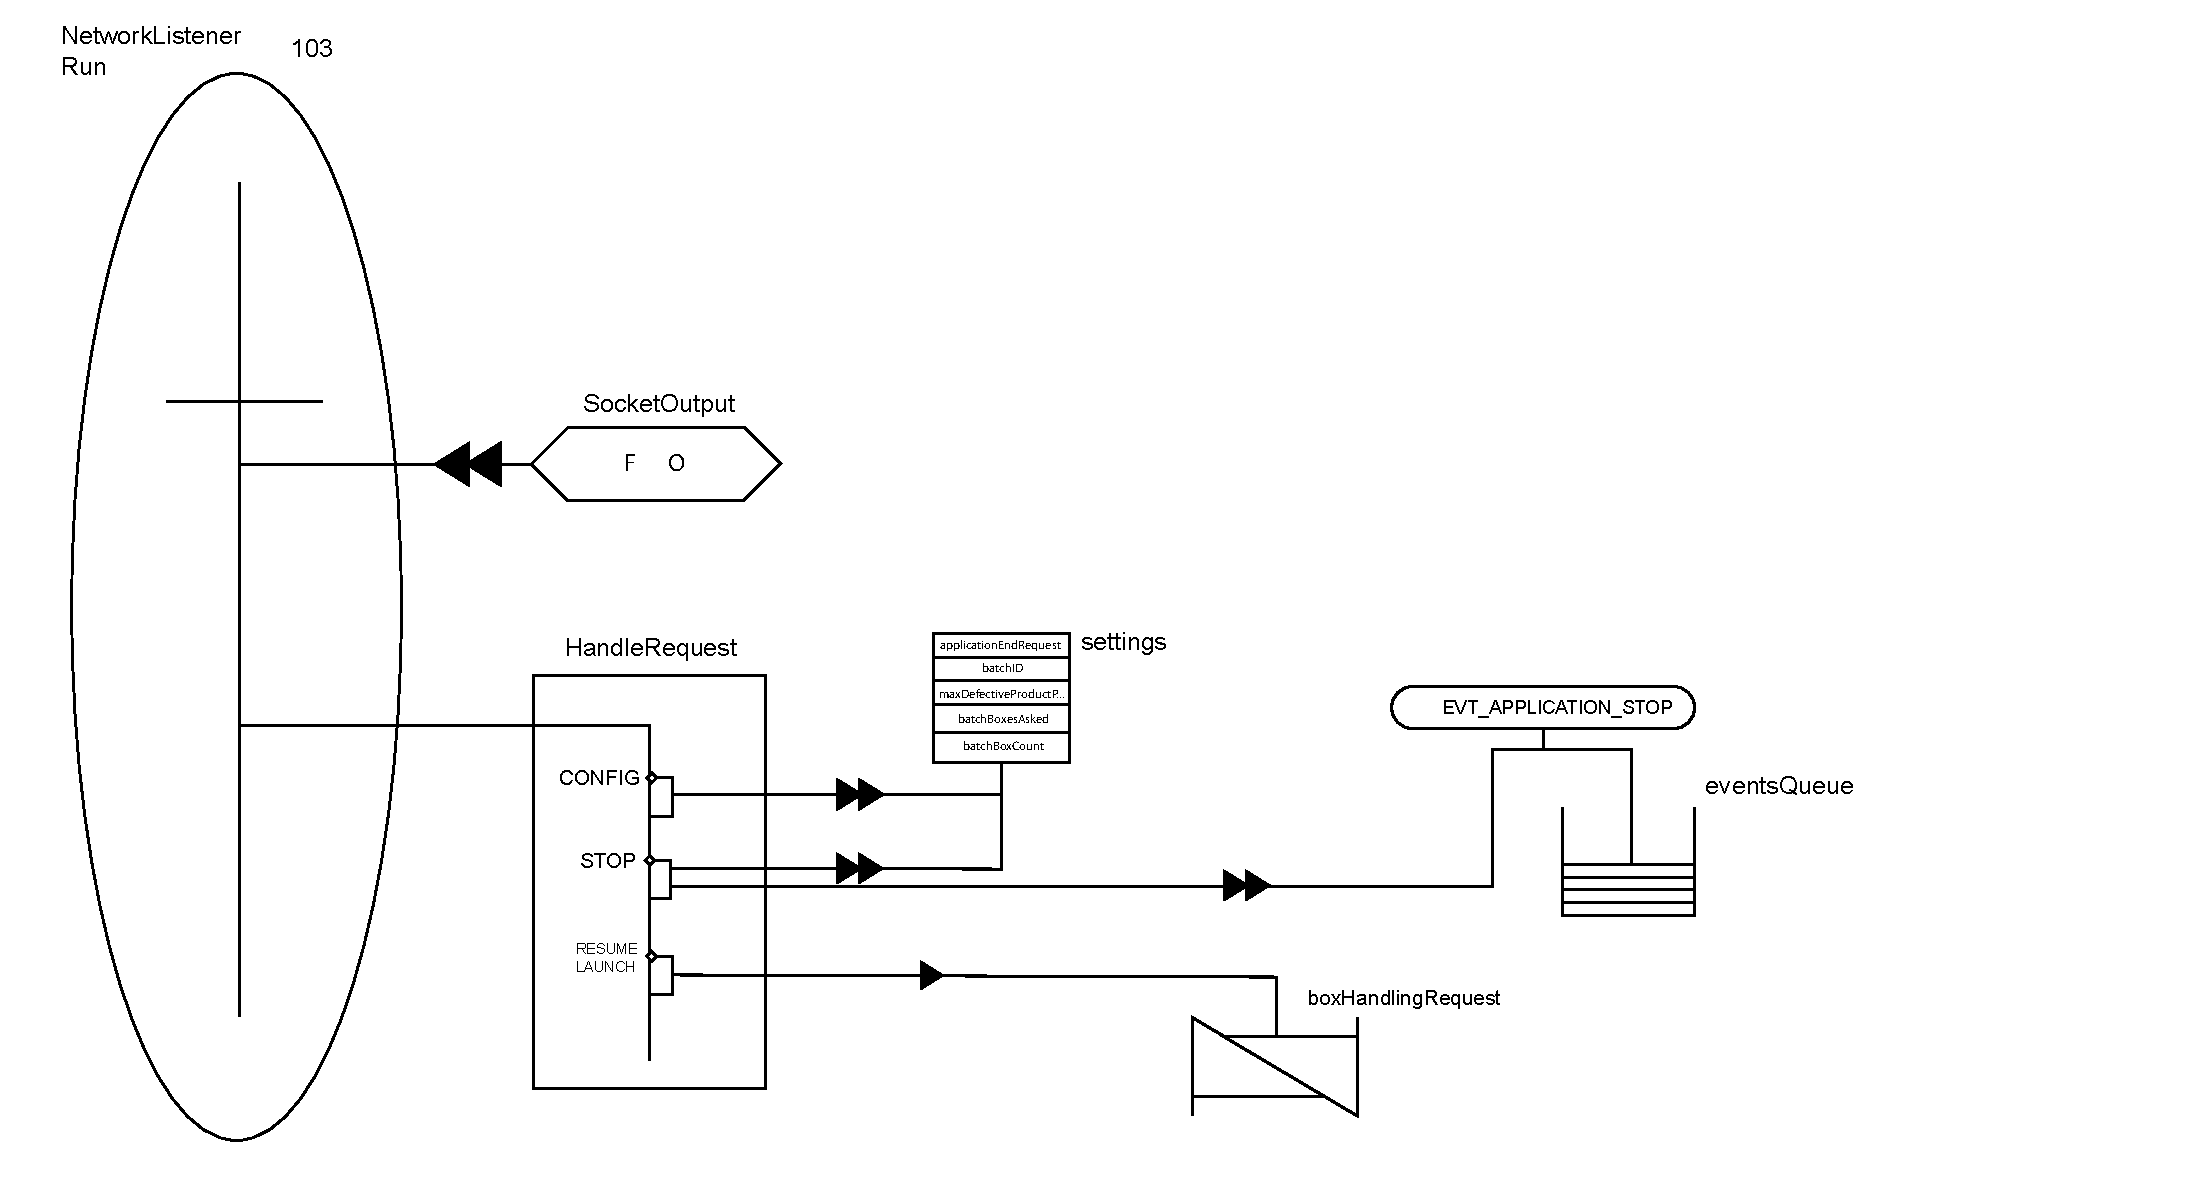
\includegraphics[width=\textwidth]{../SchemasLCG/NetworkListener-run.pdf}

	\end{frame}

	

	\begin{frame}

	\frametitle{Protocole en sortie}

	    \begin{enumerate}

	    \item \texttt{REJECTED} : nombre de pièces ayant un défaut.

	    \item \texttt{ACCEPTED} : un carton a été accepté par le système. Un argument pour indiquer le nombre de pièces.

	    \item \texttt{LOG} : l'argument est un message à afficher.

	    \item \texttt{ERROR} : erreur critique nécessitant une intervention. Un argument pour le code d'erreur.

	    \item \texttt{WARNING} : erreur non critique (panne d'imprimante).

	    \end{enumerate}

	\end{frame}

	

	\begin{frame}

	    \frametitle{LCG : EventManager : réseau en sortie}

	    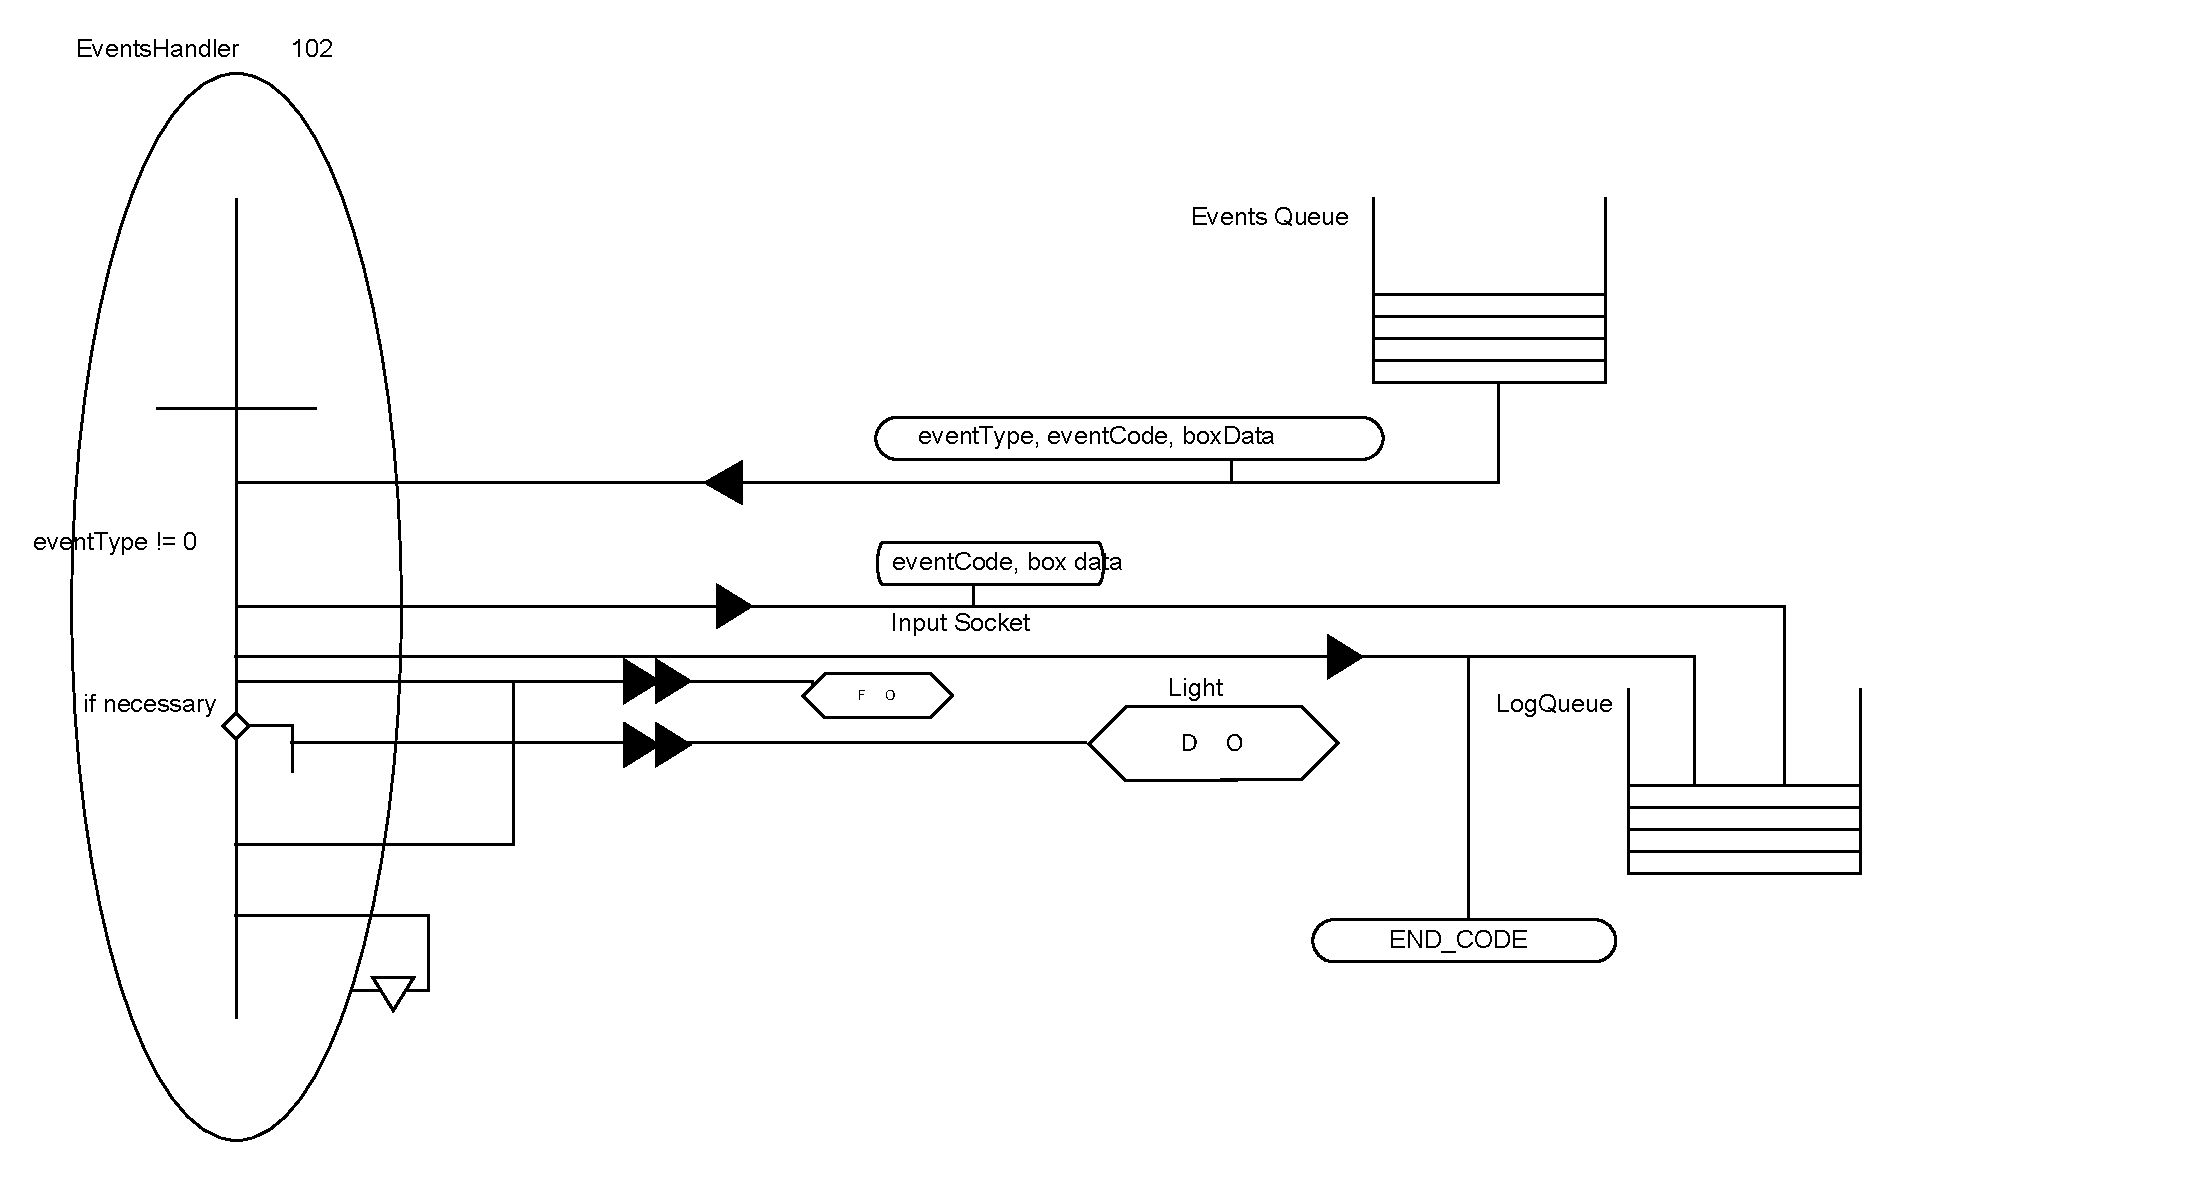
\includegraphics[width=\textwidth]{../SchemasLCG/src/EventsManager.pdf}

	\end{frame}

	

	

	\begin{frame}

	    \frametitle{LCG : Journalisation sur disque}

	    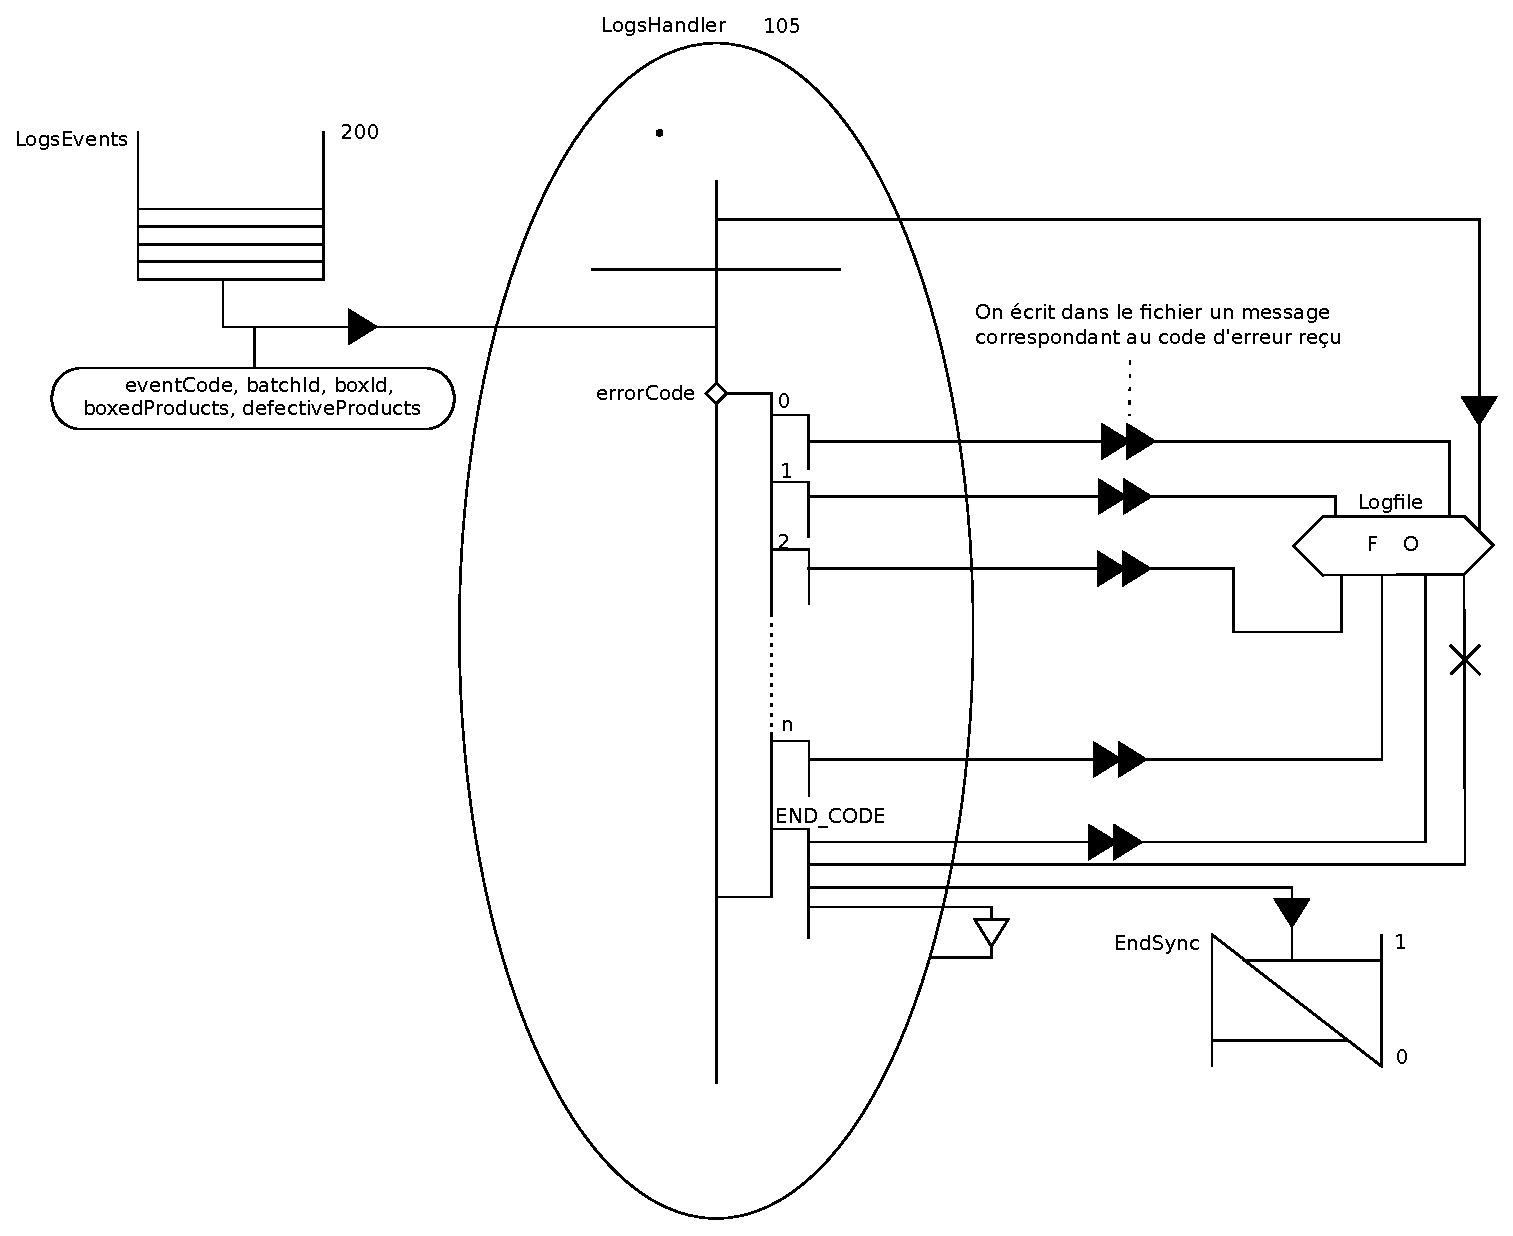
\includegraphics[width=\textwidth]{../SchemasLCG/LogsManager.pdf}

	\end{frame}

	

	\begin{frame}

	Binôme 2

	- LCG détaillé et complet en mode simulation

	\end{frame}

	

	\begin{frame}

	Binôme 2

	- justification des choix effectués pour la simulation  

	\end{frame}

\section{Binôme 3 (Martin, Etienne)}
	\begin{frame}
	\begin{center}
		\huge Lot 3 : TODO décrire
		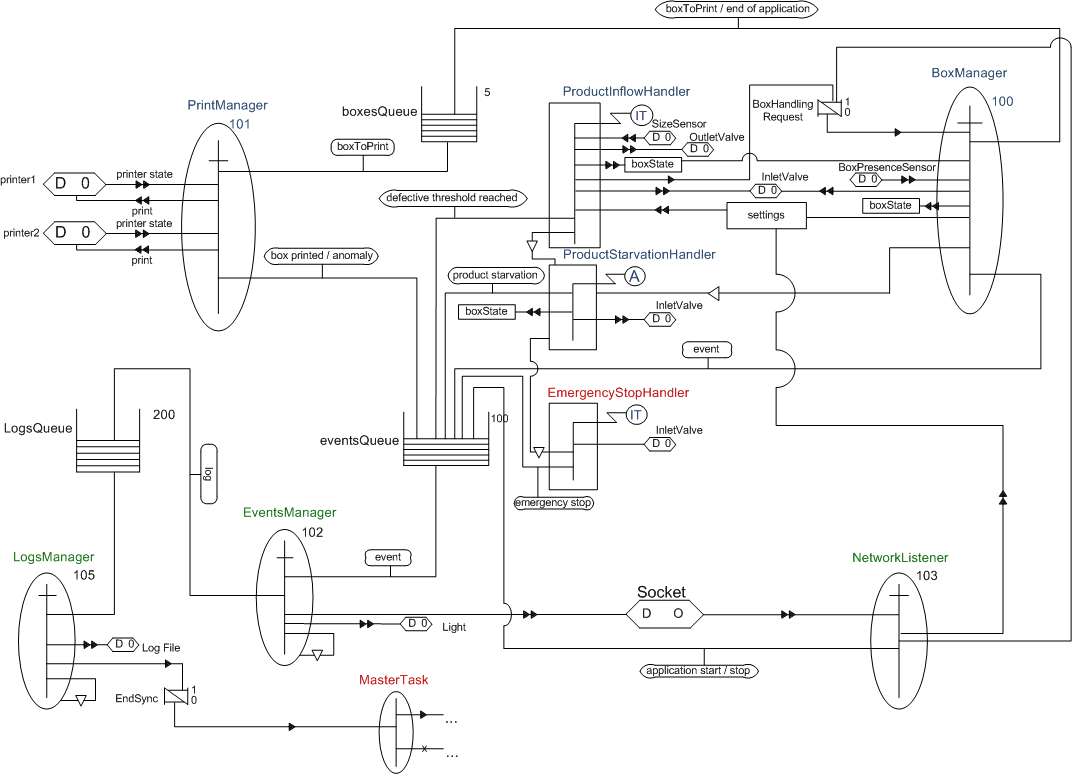
\includegraphics[height=0.8\textheight]{../../SchemasLCG/schemaGlobal.png}
	\end{center}
	\end{frame}

	\begin{frame}
		LCG détaillé et complet en mode simulation
	\end{frame}

	\begin{frame}
		justification des choix effectués pour la simulation 
	\end{frame}

\section{Intégration}
	\begin{frame}
		Intégration
		\begin{itemize}
			\item démarche
			\item plan
			\item tests
			\item resultats
		\end{itemize}
		%TODO
	\end{frame}

	\begin{frame}
		démonstration de vos réalisations
		%TODO démonstration externe au slides ?
	\end{frame}

	\begin{frame}
		bilan du projet
		\begin{itemize}
			\item auto-critique
			\item améliorations possibles
			\item points forts/faibles
			\item difficultés rencontrées ...
		\end{itemize}
		%TODO
	\end{frame}

\end{document}

